\paragraph{Ex (4.1.11)} Hur snabbt förändras volymen av en rektangulär
låda då höjden är $6$ cm, bredden är $5$ cm och djupet är $4$ cm om både
höjd och djup ökar med $1$ cm/s och bredden minskar med $2$ cm/s?
\subparagraph{Lösning} Rita!\\
%infoga bild 1
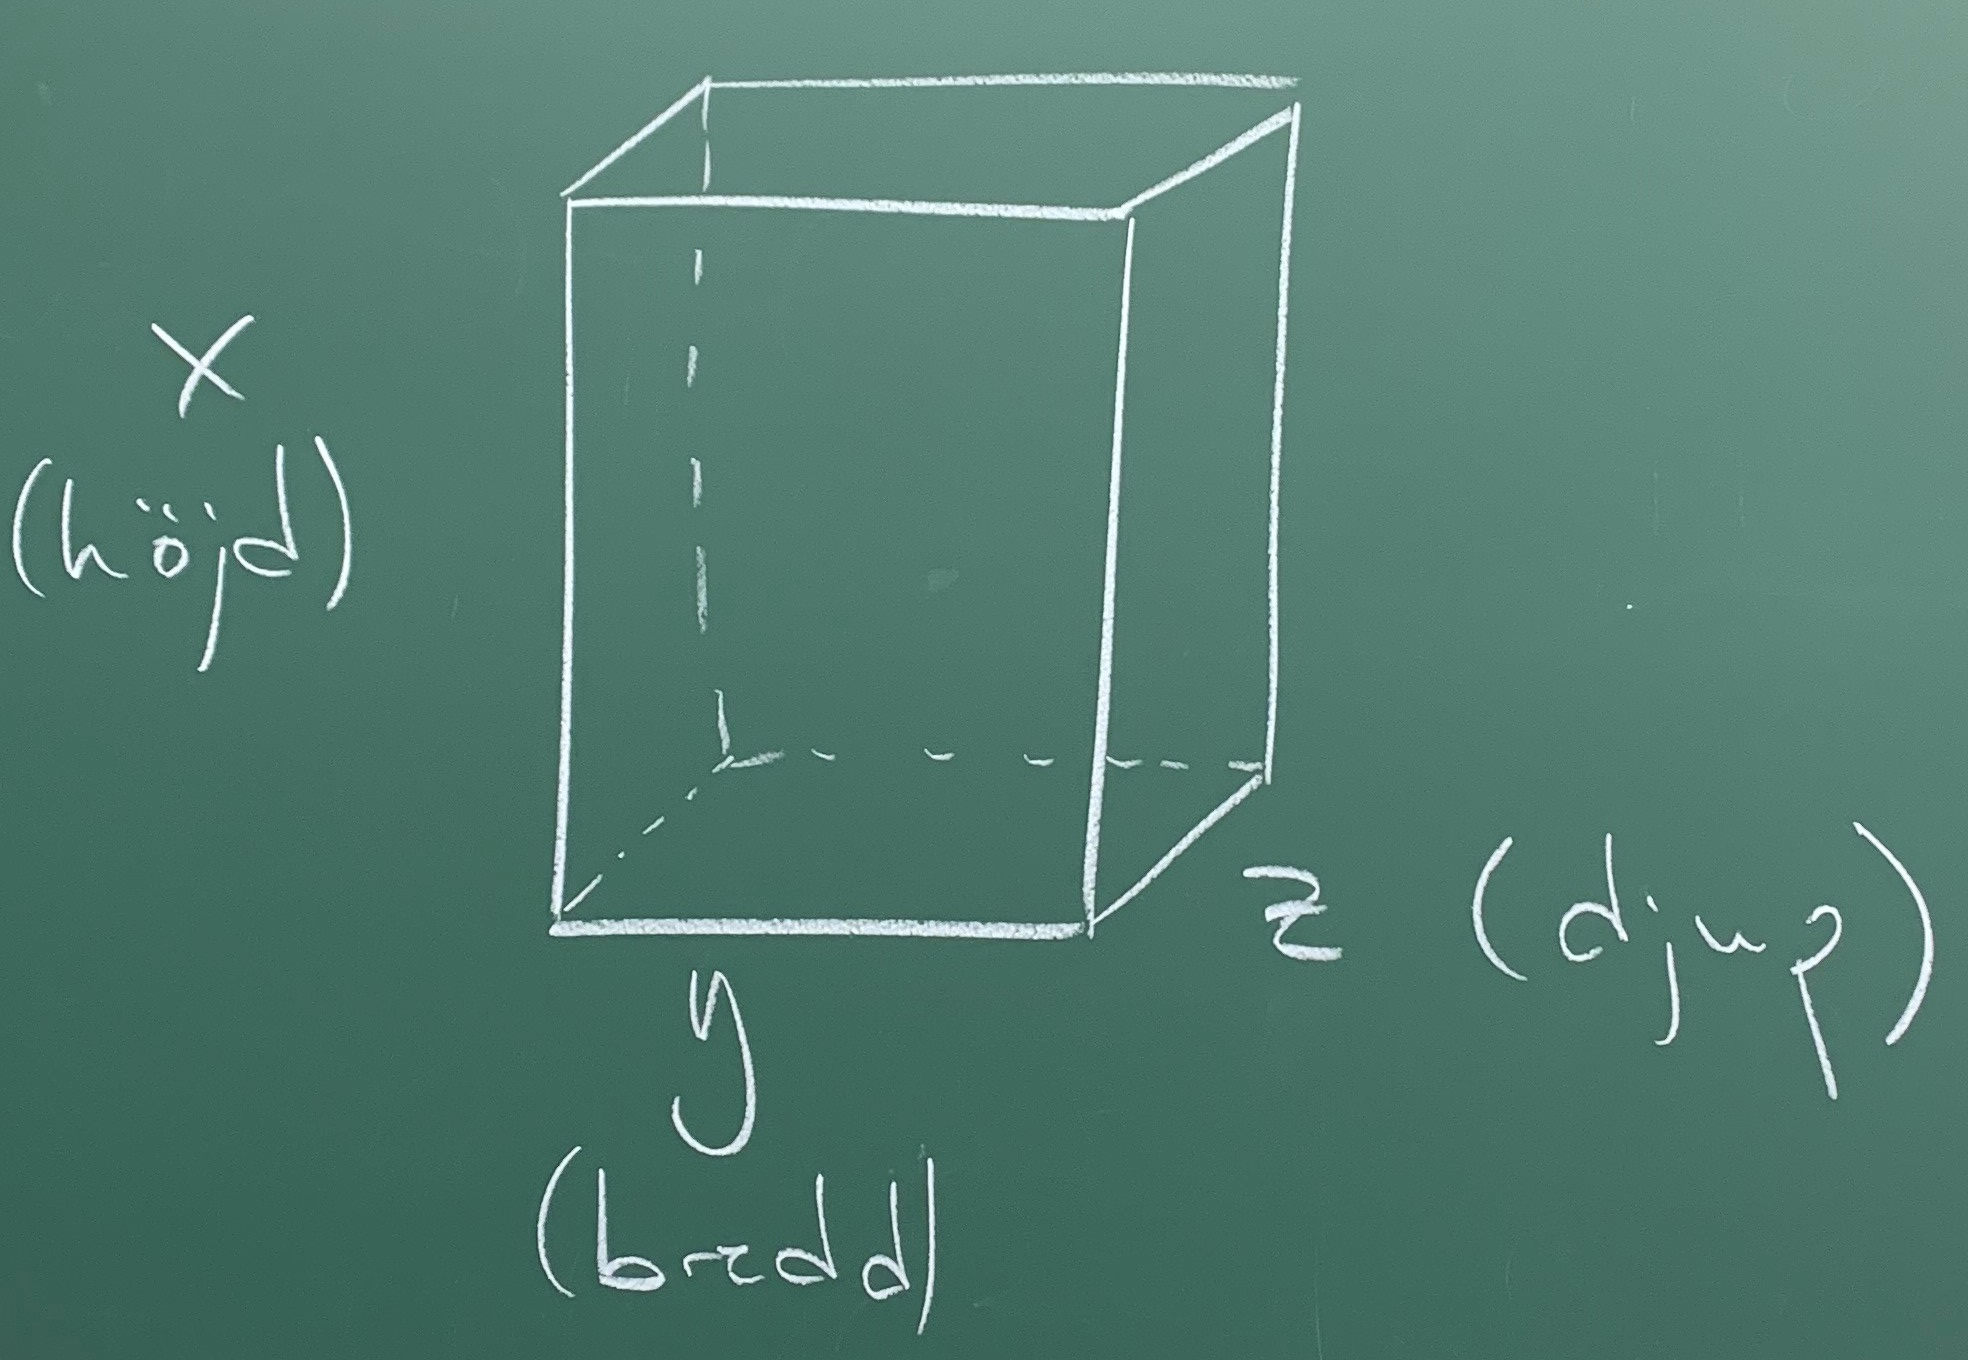
\includegraphics[scale=0.1]{lessons/lesson10/imgs/img01.jpg}\\
Lådans dimensioner beror av tiden så $x=x(t)$, $y=y(t)$ och $z=z(t)$.
Det gäller för volymen $V(t)$ att $V(t)=x(t)\cdot y(t)\cdot z(t)$
och vid tiden $t=t_0$ vet vi att $x(t_0)=6,y(t_0)=5,z(t_0)=4,x^\prime(t_0)=<^\prime(t_0)=1$ och $y^\prime(t_0)=-2$.
Vad blir $V^\prime(t_0)$?
\begin{equation*}
    V^\prime(t)=\frac{d}{dt}(x(t)\cdot y(t)\cdot z(t))=
    \{\text{prod.regeln}\}=
\end{equation*}
\begin{equation*}
    x^\prime(t)\cdot y(t)\cdot z(t) + x(t)\cdot y^\prime(t)\cdot z(t) + x(t)\cdot y(t)\cdot z^\prime(t)
    \Rightarrow V^\prime(t_0)=
\end{equation*}
\begin{equation*}
    1\cdot 5\cdot 4 + 6\cdot (-2)\cdot 4 + 6\cdot 5 \cdot 1=
    20-48+30=2\text{ cm}^3\text{/s}
\end{equation*}
så lådans volym \underline{ökar} med $2$ cm$^3$/s $\Box$

\paragraph{Ex (4.1.38)} Två tunga lådor är sammankopplade med ett $15$ m långt och starkt (icke-elastiskt) rep enligt figur\\
%infoga bild 2
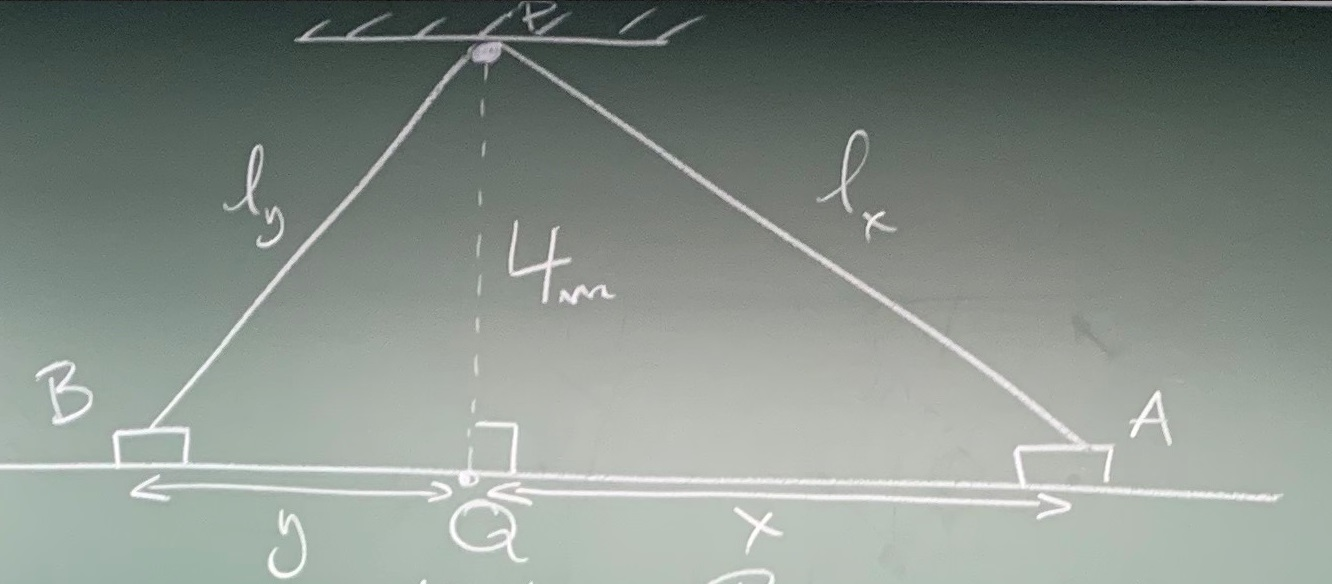
\includegraphics[scale=0.1]{lessons/lesson10/imgs/img02.jpg}\\
Hur snabbt rör sig låda $B$ mot punkten $Q$ då låda $A$ befinner sig $3$ m
från $Q$ och rör sig bort från denna punkt med en fart av $0.5$ m/s?
\subparagraph{Lösning}
Beteckna repets längd $l$ och de båda dellängderna $l_x$ och $l_y$.\\
Då gäller att:
$l(t)=l_x(t)+l_y(t)=\sqrt{x^2(t)+4^2}+\sqrt{y^2(t)+4^2}$ och
\begin{equation*}
    0=l^\prime(t)=\frac{1}{2}(x^2(t)+16)^{-\frac{1}{2}}\cdot 2x(t)\cdot x^\prime(t)+\frac{1}{2}(y^2(t)+16)^{-\frac{1}{2}}\cdot 2y(t)\cdot y^\prime(t)=
\end{equation*}
\begin{equation*}
    \frac{x(t)\cdot x^\prime(t)}{\sqrt{x^2(t)+16}}+\frac{y(t)\cdot y^\prime(t)}{\sqrt{y^2(t)+16}}
\end{equation*}
Vi vet att vid $t=t_0$ så är $x(t_0)=3,x^\prime(t_0)=0.5$ och \\
$y(t_0)=\sqrt{l_y^2-16}=\sqrt{(l-l_x)^2-16}=\sqrt{(15-\sqrt{16-9})^2-16}=\sqrt{84}$så \\
$0=\frac{3\cdot 0.5}{\sqrt{9+16}}+\frac{\sqrt{84}\cdot y^\prime(t_0)}{\sqrt{84+16}}\Rightarrow y^\prime(t_0)=-\frac{3}{\sqrt{84}}\approx -0.327\text{m/s }\Box$

\chapter{Numerisk ekvationslösning}
Handlar om att på numerisk väg lösa ekvationen $f(x)=0$.
Om till exempel $f$ är kontinuerlig kan man anvönda \underline{bisektionsalgoritmen}, dvs. hitta två tal $a$ och $b$ så att $f(a)<0$ och $f(b)>0$ (eller tvärt om!).
Då ligger åtminstone ett nollställe mellan $a$ och $b$.
Beräkna $f(\frac{a+b}{2})$, dvs. värdet i mittpunkten och avgör sedan om nollställe ligger i antingen intervallet $[a,\frac{a+b}{2}]$ eller i $[\frac{a+b}{2}, b]$.
Fortsätt på samma vis i delintervallen\dots

\paragraph{Fixpunktsiteration} Formulera om $f(x)=0$ som $g(x)=x$ (om möjligt).
Till exempel $f(x)=3\sin^2(x)+x^2-x=0$ blir då $g(x)=3\sin^2(x)+x^2=x$.
Tag sedan ett tal $x=x_0$ som troligtvis ligger nära det $x$ som löser ekvationen och sätt in i $g(x)$.
$x_0\rightarrow g(x_0)=x_1\rightarrow g(x_1)=x_2\rightarrow g(x_2)...$ dvs. beräkna $x_0,x_1,x_2,...$ enligt $g(x_n)=x_{n+1}$.
Under vissa förutsättningar konvergerar talföljden $\lim_{n\to\infty}x_n$ och man hittar en lösning till $g(x)=x$ dvs. $f(x)=0$.
Gränsvärdet $lim_{n\to\infty}x_n=x$ kallas \underline{fixpunkt} till $g(x)$.

\paragraph{Sats} Antag att $g$ är definierad på intervallet $I=[a,b]$ och uppfyllet att:
\begin{enumerate}
    \item $f(x)\in I$ om $x\in I$
    \item Det finns en konstant $0<k<1$ så att för att $u,v\in I$ gäller att $|f(u)-f(v)|\leq k\cdot|u-v|$ (lipschitz-kontinuitet).
          Då har $g$ en unik fixpunkt $r\in I$, dvs. $g(r)=r$, och oavsett val av $x_0\in I$ så är $\lim_{n\to\infty}x_n=r$.
\end{enumerate}

\paragraph{Newtons metod} Funkar bra om man söker nollställen $f(x)=0$ där $f$ är en deriverbar funktion.
Går ut på att iterativt hitta nollställen till tangentlinjer!\\
%infoga bild 3
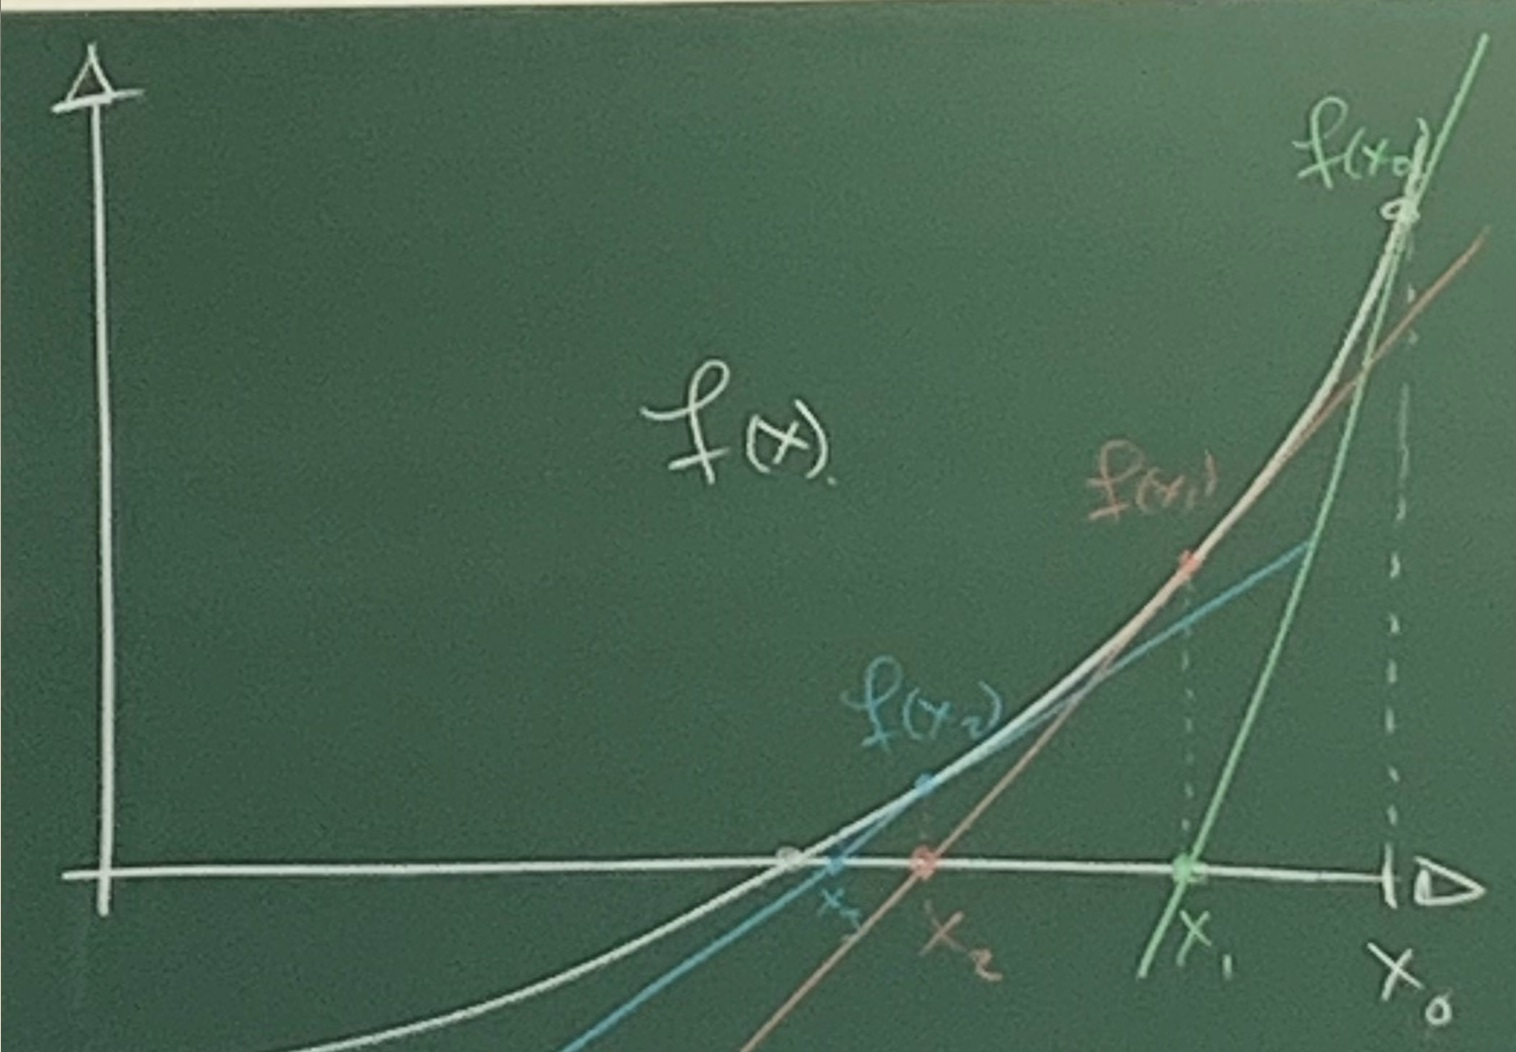
\includegraphics[scale=0.1]{lessons/lesson10/imgs/img03.jpg}\\
För $x=x_n$ har man tangentlinjen $\frac{y-f(x_n)}{x-x_n}=f^prime(x_n)$ och nollstället till denna ges av $\frac{0-f(x_n)}{x_{n+1}-x_n}=f^\prime(x_n)$ dvs $x_{n+1}=x_n-\frac{f(x_n)}{f^\prime(x_n)}$.
Newtons metod kan fallera om $f$ inte ör överallt deriverbar eller om det finns horizontella/vertikala tangenter.

\chapter{Extremvärden}
Ett extremvärde av en funktion $f$ är en punkt där värdet av $f$ är \\
maximalt/minimalt, antingen globalt eller lokalt.

\paragraph{Definition (globalt extremvärde)} En funktion $f$ har ett eller flera globalt maximum/minimum i $x=x_0$ (där $x_0\in D(f)$) om $f(x)\begin{matrix}\geq\\\leq\end{matrix}f(x_0)$ för alla $x\in D(f)$.

\paragraph{Definition (lokalt extremvärde)} En funktion $f$ har ett lokalt \\
maximum/minimum i $x=x_0$ (där $x_0\in D(f)$) om det finns ett tal $h>0$ så att $f(x)\begin{matrix}\geq\\\leq\end{matrix} f(x_0)$ för att $x\in D(f)$ så att $|x-x_0|<h$.\\
I en bild:\\
%ingoga bild 4
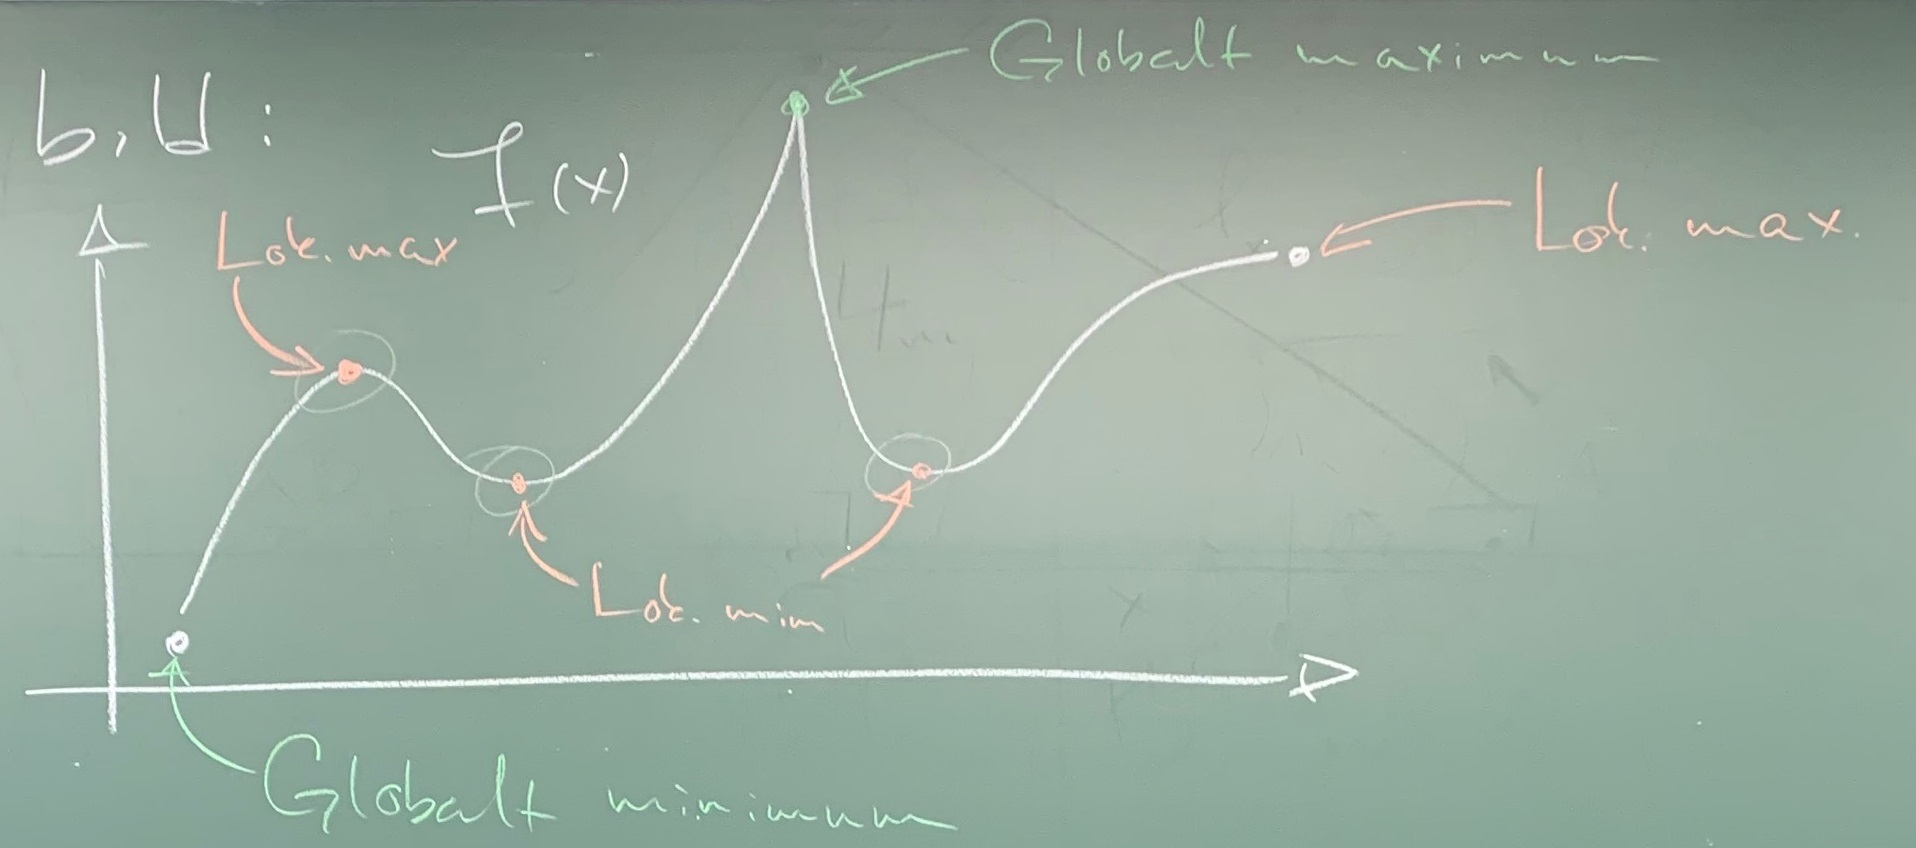
\includegraphics[scale=0.1]{lessons/lesson10/imgs/img04.jpg}\\
Lokala (och globala) extrempunkter kan hittas i tre olika typer av fall:
\begin{enumerate}
    \item Kritiska punkter, dvs. i $x$ sådana att $f^\prime(x)=0$.
    \item Singulär punkter, dvs i $x$ sådana att $f^\prime(x)$ ej existerar.
    \item Ändpunkter av $D(f)$
\end{enumerate}

\paragraph{Ex (4.4.13)} Hitta alla globala och lokala extrempunkter till $f(x)= |x-1|$, $x\in[-2,2]$
\subparagraph{Lösning} $f$ saknar kritiska punkter (eftersom $f^\prime(x)=sgn(x-1)$).
Har singulär punkt i $x=1$ där $f(1)=0$ och i ändpunkterna gäller att:
\begin{itemize}
    \item $f(-2)= | -2-1| = | -3|=3$
    \item $f(2)= | 2-1| = |1| = 1$
\end{itemize}
så globalt minimum i $x=1$, globalt maximum i $x=-2$ och lokalt maximum i $x=2$.\\
%infoga bild 5
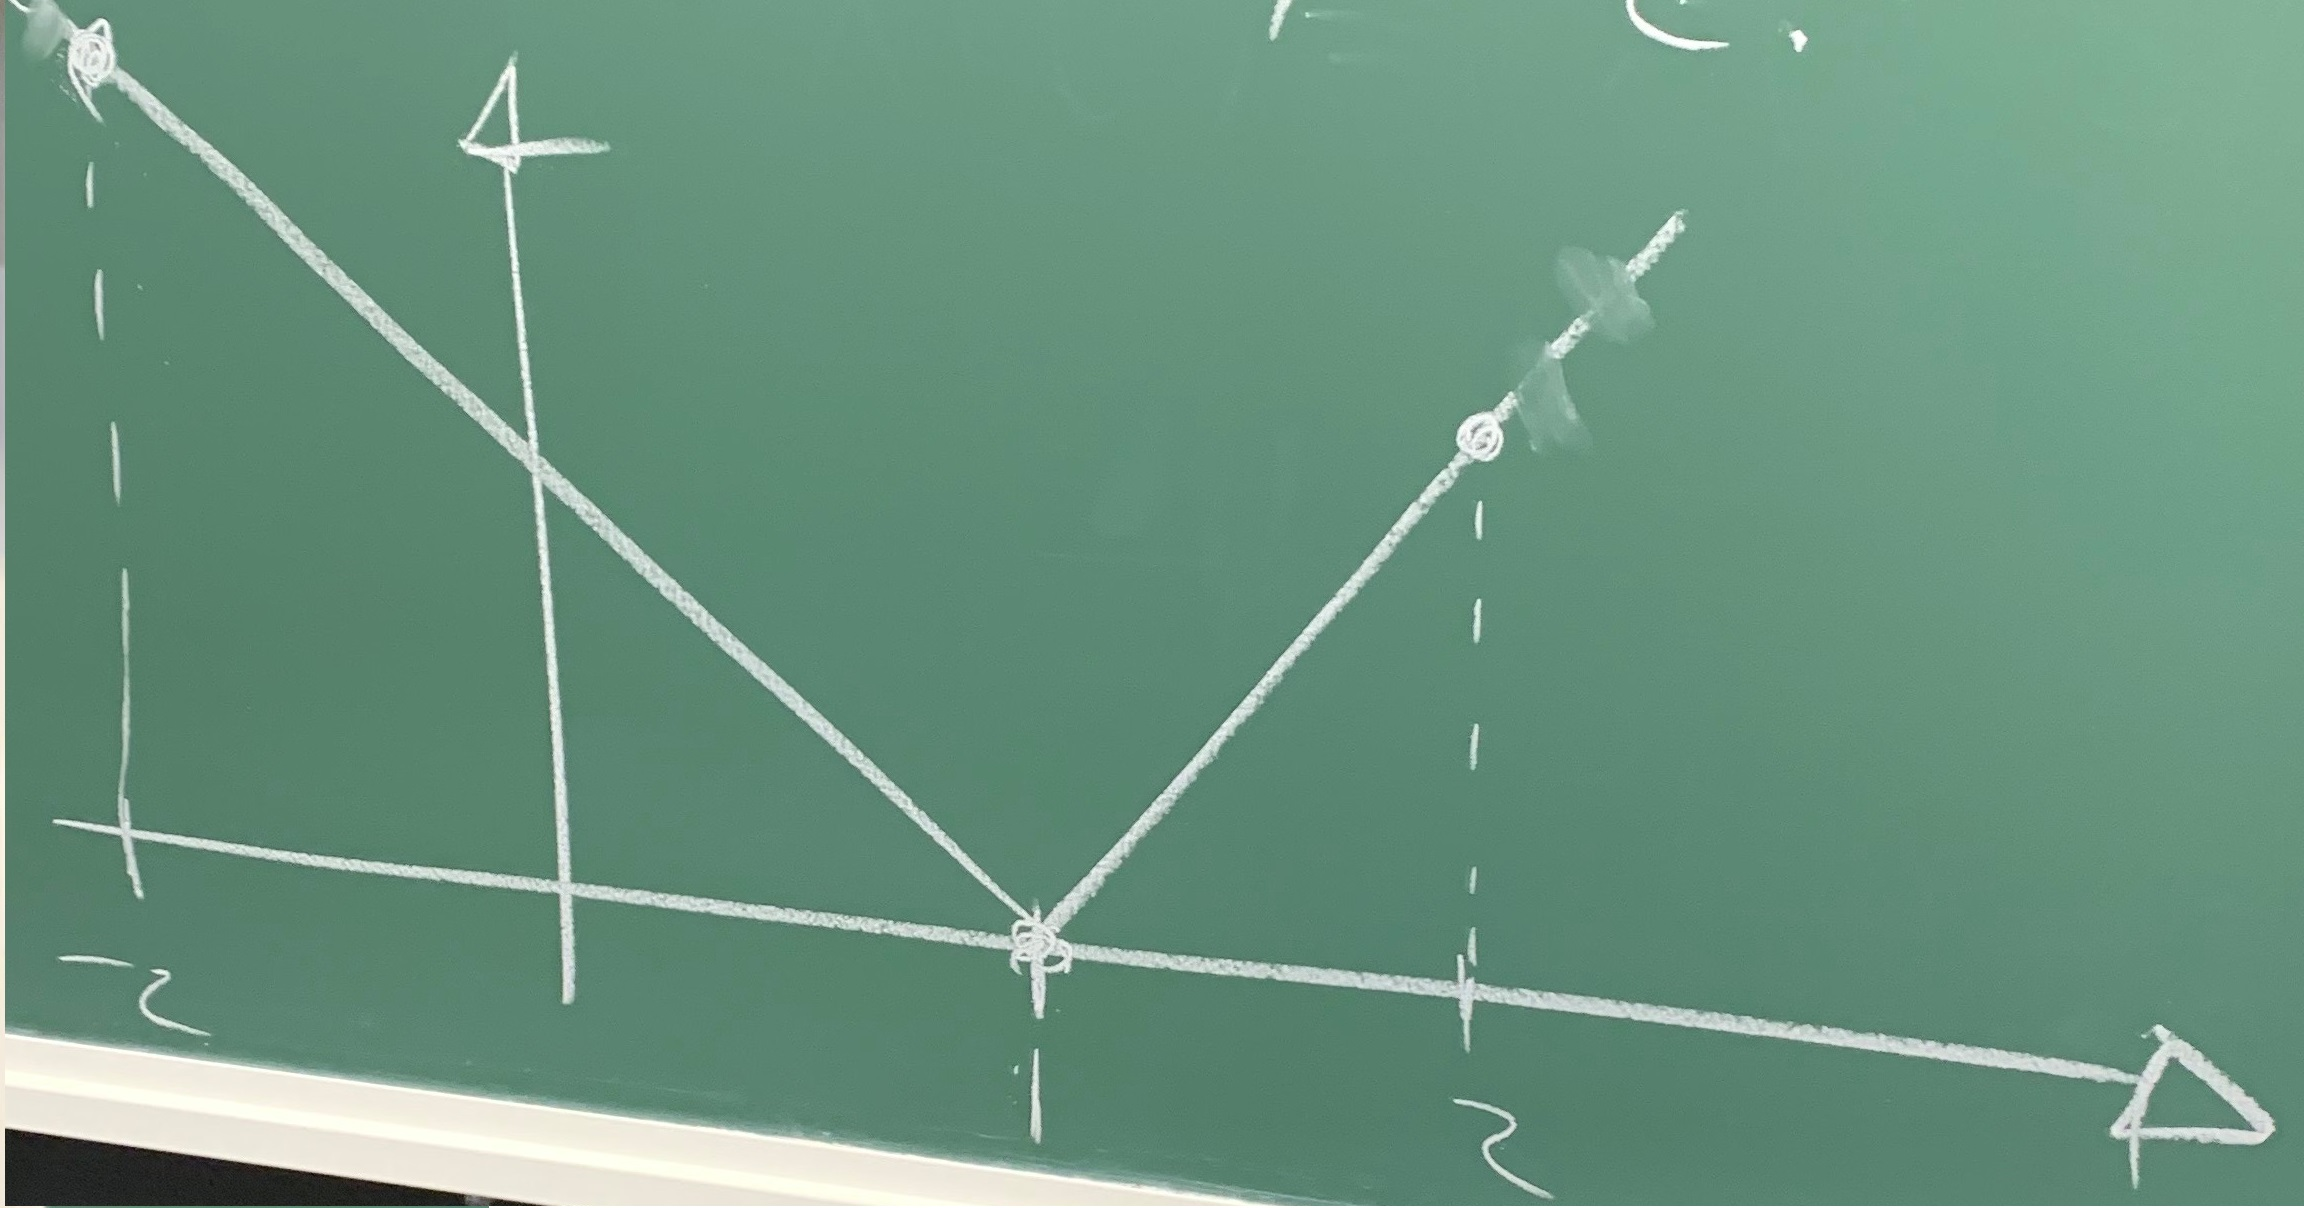
\includegraphics[scale=0.1]{lessons/lesson10/imgs/img05.jpg}\\
